%package list
\documentclass{article}
\usepackage[top=3cm, bottom=3cm, outer=3cm, inner=3cm]{geometry}
\usepackage{multicol}
\usepackage{graphicx}
\usepackage{url}
%\usepackage{cite}
\usepackage{hyperref}
\usepackage{array}
%\usepackage{multicol}
\newcolumntype{x}[1]{>{\centering\arraybackslash\hspace{0pt}}p{#1}}
\usepackage{natbib}
\usepackage{pdfpages}
\usepackage{multirow}    
\usepackage[normalem]{ulem}
\useunder{\uline}{\ul}{}
\usepackage{svg}
\usepackage{xcolor}
\usepackage{listings}
\lstdefinestyle{ascii-tree}{
    literate={├}{|}1 {─}{--}1 {└}{+}1 
  }

\lstset{basicstyle=\ttfamily,
  showstringspaces=false,
  commentstyle=\color{red},
  keywordstyle=\color{blue}
}
%\usepackage{booktabs}
\usepackage{caption}
\usepackage{subcaption}
\usepackage{float}
\usepackage{array}

\usepackage{enumitem}


\newcolumntype{M}[1]{>{\centering\arraybackslash}m{#1}}
\newcolumntype{N}{@{}m{0pt}@{}}


%%%%%%%%%%%%%%%%%%%%%%%%%%%%%%%%%%%%%%%%%%%%%%%%%%%%%%%%%%%%%%%%%%%%%%%%%%%%
%%%%%%%%%%%%%%%%%%%%%%%%%%%%%%%%%%%%%%%%%%%%%%%%%%%%%%%%%%%%%%%%%%%%%%%%%%%%
\newcommand{\itemEmail}{vmaldonadov@unsa.edu.pe, acunoc@unsa.edu.pe}
\newcommand{\itemStudent}{Victor Gonzalo Maldonado Vilca, Armando Steven Cuno Cahuari}
\newcommand{\itemCourse}{Estructura de Datos y Algoritmos}
\newcommand{\itemCourseCode}{1702122}
\newcommand{\itemSemester}{III}
\newcommand{\itemUniversity}{Universidad Nacional de San Agustín de Arequipa}
\newcommand{\itemFaculty}{Facultad de Ingeniería de Producción y Servicios}
\newcommand{\itemDepartment}{Departamento Académico de Ingeniería de Sistemas e Informática}
\newcommand{\itemSchool}{Escuela Profesional de Ingeniería de Sistemas}
\newcommand{\itemAcademic}{2024 - A}
\newcommand{\itemInput}{Del 11/07/2024 -- 00:00am}
\newcommand{\itemOutput}{Al 11/07/2024 -- 23:59pm}
\newcommand{\itemPracticeNumber}{08}
\newcommand{\itemTheme}{Algoritmo de Compresión de Huffman}
%%%%%%%%%%%%%%%%%%%%%%%%%%%%%%%%%%%%%%%%%%%%%%%%%%%%%%%%%%%%%%%%%%%%%%%%%%%%
%%%%%%%%%%%%%%%%%%%%%%%%%%%%%%%%%%%%%%%%%%%%%%%%%%%%%%%%%%%%%%%%%%%%%%%%%%%%

\usepackage[english,spanish]{babel}
\usepackage[utf8]{inputenc}
\AtBeginDocument{\selectlanguage{spanish}}
\renewcommand{\figurename}{Figura}
\renewcommand{\refname}{Referencias}
\renewcommand{\tablename}{Tabla} %esto no funciona cuando se usa babel
\AtBeginDocument{%
	\renewcommand\tablename{Tabla}
}

\usepackage{fancyhdr}
\pagestyle{fancy}
\fancyhf{}
\setlength{\headheight}{30pt}
\renewcommand{\headrulewidth}{1pt}
\renewcommand{\footrulewidth}{1pt}
\fancyhead[L]{\raisebox{-0.2\height}{
\includegraphics[width=3cm]{img/logo_episunsa.png}}}
\fancyhead[C]{\fontsize{7}{7}\selectfont	\itemUniversity \\ \itemFaculty \\ \itemDepartment \\ \itemSchool \\ \textbf{\itemCourse}}
\fancyhead[R]{\raisebox{-0.2\height}{
\includegraphics[width=1.2cm]{img/logo_abet}}}
\fancyfoot[L]{Victor M.}
\fancyfoot[C]{\itemCourse}
\fancyfoot[R]{Página \thepage}

% para el codigo fuente
\usepackage{listings}
\usepackage{color, colortbl}
\definecolor{dkgreen}{rgb}{0,0.6,0}
\definecolor{gray}{rgb}{0.5,0.5,0.5}
\definecolor{mauve}{rgb}{0.58,0,0.82}
\definecolor{codebackground}{rgb}{0.95, 0.95, 0.92}
\definecolor{tablebackground}{rgb}{0.8, 0, 0}

\lstset{frame=tb,
	language=bash,
	aboveskip=3mm,
	belowskip=3mm,
	showstringspaces=false,
	columns=flexible,
	basicstyle={\small\ttfamily},
	numbers=none,
	numberstyle=\tiny\color{gray},
	keywordstyle=\color{blue},
	commentstyle=\color{dkgreen},
	stringstyle=\color{mauve},
	breaklines=true,
	breakatwhitespace=true,
	tabsize=3,
	backgroundcolor= \color{codebackground},
}

\begin{document}
	
	\vspace*{10px}
	
	\begin{center}	
		\fontsize{17}{17} \textbf{ Informe de Laboratorio 08 }
	\end{center}
	\centerline{\textbf{\Large Tema: \itemTheme}}
	%\vspace*{0.5cm}	

	\begin{flushright}
		\begin{tabular}{|M{2.5cm}|N|}
			\hline 
			\rowcolor{tablebackground}
			\color{white} \textbf{Nota}  \\
			\hline 
			     \\[30pt]
			\hline 			
		\end{tabular}
	\end{flushright}	

	\begin{table}[H]
		\begin{tabular}{|x{4.7cm}|x{4.8cm}|x{4.8cm}|}
			\hline 
			\rowcolor{tablebackground}
			\color{white} \textbf{Estudiante} & \color{white}\textbf{Escuela}  & \color{white}\textbf{Asignatura}   \\
			\hline 
			{\itemStudent \par \itemEmail} & \itemSchool & {\itemCourse \par Semestre: \itemSemester \par Código: \itemCourseCode}     \\
			\hline 			
		\end{tabular}
	\end{table}		
	
	\begin{table}[H]
		\begin{tabular}{|x{4.7cm}|x{4.8cm}|x{4.8cm}|}
			\hline 
			\rowcolor{tablebackground}
			\color{white}\textbf{Tarea} & \color{white}\textbf{Tema}  & \color{white}\textbf{Duración}   \\
			\hline 
			\itemPracticeNumber & \itemTheme & 2 horas   \\
			\hline 
		\end{tabular}
	\end{table}
	
	\begin{table}[H]
		\begin{tabular}{|x{4.7cm}|x{4.8cm}|x{4.8cm}|}
			\hline 
			\rowcolor{tablebackground}
			\color{white}\textbf{Semestre académico} & \color{white}\textbf{Fecha de inicio}  & \color{white}\textbf{Fecha de entrega}   \\
			\hline 
			\itemAcademic & \itemInput &  \itemOutput  \\
			\hline 
		\end{tabular}
	\end{table}
%%%%%%%%%%%%%%%%%%%%

  \section{Introducción}
  \begin{enumerate}
    \item Algoritmo de compresión de Huffman
    \begin{itemize}
      \item Se trata de un algoritmo que puede ser usado para compresión o encriptación de datos. Este algoritmo 
      se basa en asignar códigos de distinta longitud de bits a cada uno de los caracteres de un fichero. 
      \item Si se asignan códigos más cortos a los caracteres que aparecen más a menudo se consigue una compresión del fichero.
      \item Esta compresión es mayor cuando la variedad de caracteres diferentes que aparecen es menor.
    \end{itemize}
    Por ejemplo: si el texto se compone  únicamente de números o mayúsculas, se conseguirá una compresión mayor.
    Para recuperar el fichero original es necesario conocer el código asignado a cada caracter, así como su longitud en bits, 
    si  ésta información se omite, y el receptor del fichero la conoce, podrá recuperar la información original. De este modo 
    es posible utilizar el algoritmo para encriptar ficheros.
    \item Mecanismo del algoritmo
    \begin{itemize}
      \item Contar cuantas veces aparece cada caracter en el fichero a comprimir. Y crear una lista enlazada con la 
      información de caracteres y frecuencias.
      \item Ordenar la lista de menor a mayor en función de la frecuencia.
      \item Convertir cada elemento de la lista en un árbol.
      \item Fusionar todos estos  árboles en uno  único, para hacerlo se sigue el siguiente proceso, mientras la lista de 
      árboles contenga más de un elemento:
      \item -------• Con los dos primeros árboles formar un nuevo  árbol, cada uno de los  árboles originales en una rama.
      \item -------• Sumar las frecuencias de cada rama en el nuevo elemento árbol.
      \item -------• Insertar el nuevo  árbol en el lugar adecuado de la lista según la suma de frecuencias obtenida.
      \item Para asignar el nuevo código binario de cada caracter sólo hay que seguir el camino adecuado através del árbol. 
      \item Si se toma una rama cero, se añade un cero al código, si se toma una rama uno, se añade un uno.
      \item Se recodifica el fichero según los nuevos códigos.
    \end{itemize}
    \item Veamos un ejemplo \textbf{Tomemos un texto corto, por ejemplo: \textit{"ata la jaca a la estaca”}}
    \begin{enumerate}
      \item Contamos las veces que aparece cada caracter y hacemos una lista enlazada: ’  ’(5), a(9), c(2), e(1), j(1), 
      l(2), s(1), t(2).
      \item Ordenamos por frecuencia de menor a mayor: e(1), j(1), s(1), c(2), l(2), t(2), ’  ’(5), a(9).
      \item Consideremos ahora que cada elemento es el nodo raíz de un árbol.
      \item Fusionamos los dos primeros nodos ( árboles) en un nuevo  árbol, sumamos sus frecuencias y lo colocamos 
      en el lugar correspondiente:
      \item Asignamos los códigos, las ramas a la izquierda son ceros, y a la derecha unos, es una regla arbitraria.
    \end{enumerate}
  \end{enumerate}

%%%%%%%%%%%%%%%%%%%%

  \section{Objetivos}
  \begin{itemize}
    \item Comprender y aplicar el algoritmo de compresión de Huffman.
    \item Implementar el algoritmo en un lenguaje de programación.
    \item Analizar la eficiencia del algoritmo.
    \item Documentar el proceso de implementación.
  \end{itemize}

%%%%%%%%%%%%%%%%%%%%
 
	\section{Tarea}
  Elabore un informe paso a paso de la implementación del algoritmo de compresión mediante el algoritmo de Huffman.
 
%%%%%%%%%%%%%%%%%%%% 
 
  \section{Entregables}
  \begin{itemize}
    \item Informe hecho en Latex.
    \item URL: Respositorio GitHub.
  \end{itemize}
  
%%%%%%%%%%%%%%%%%%%%    
		
	\section{Equipos, materiales y temas utilizados}
  \begin{itemize}
    \item Teoría de la Compresión de Datos.
    \item Algoritmo de Huffman.
    \item Estructuras de Datos.
    \item Java.
  \end{itemize}
 
%%%%%%%%%%%%%%%%%%%%

  \section{URL de Repositorio Github}
  \begin{itemize}
    \item Link de Repositorio GitHub.
    \item \url{https://github.com/Victor-Gonzalo-Maldonado-Vilca/EDA_Lab08.git}
  \end{itemize}

%%%%%%%%%%%%%%%%%%%%

  \section{Desarrollo del trabajo}
  El flujo de trabajo gracias al algoritmo de Huffman permite minimizar el espacio ocupado por documentos, 
  entre otros. Para ello, es necesario hacer un recuento de la frecuencia de cada carácter. Luego, debemos 
  ordenar estos caracteres de menor a mayor frecuencia para construir el árbol Heap. A continuación, mediante 
  una iteración de ese ordenamiento, construiremos el árbol uniendo dos nodos a la vez: el hijo izquierdo con un '0' 
  y el derecho con un '1'.
  
  \subsection{Clase Node}
  \begin{itemize}
    \item \textbf{Descripción: }Definir la clase ‘Node’ es necesario para construir el árbol de Huffman utilizando una cola de prioridad 
    o una lista enlazada. Los valores se organizan en la cola de prioridad y se usarán para construir el árbol de Huffman.
    \newline
    En esta clase, tendremos como atributos privados el carácter, la frecuencia y dos nodos hijos, izquierdo y derecho. 
    La clase tendrá dos constructores: uno que recibe como parámetros la frecuencia y el carácter, y otro que además incluye 
    los valores de los hijos izquierdo y derecho.
    \item \textbf{Código: }
    \begin{lstlisting}[language=java, numbers=left, firstnumber=1, numberstyle=\color{orange}]
    public class Node {
        char ch;
        int freq;
        Node left = null, right = null;

        Node(char ch, int freq) {
            this.ch = ch;
            this.freq = freq;
        }

        Node(char ch, int freq, Node left, Node right) {
            this.ch = ch;
            this.freq = freq;
            this.left = left;
            this.right = right;
        }
    }
    \end{lstlisting}
  \end{itemize}
  
  \subsection{Clase HuffmanComparator}
  \begin{itemize}
    \item \textbf{Descripción: }Esta clase se utilizará para ordenar la cola de prioridad basada en la frecuencia de 
    los caracteres. Tendrá un método de clase llamado `compare`, que tomará como argumento dos nodos. Este método 
    comparará las frecuencias de los dos nodos y decidirá su orden. Si `a.freq \verb|<| b.freq`, entonces `a` debe venir 
    antes que `b`. Si `a.freq \verb|>| b.freq`, entonces `a` debe venir después que `b`. Finalmente, si ambas frecuencias 
    son iguales, no habrá ningún cambio.
    \item \textbf{Código: }
    \begin{lstlisting}[language=java, numbers=left, firstnumber=1, numberstyle=\color{orange}]
    import java.util.Comparator;
    
    public class HuffmanComparator implements Comparator<Node> {
        @Override
        public int compare(Node a, Node b) {
            return a.freq - b.freq;
        }
    }
    \end{lstlisting}
  \end{itemize}
  
  \subsection{Clase HuffmanCoding}
  \begin{itemize}
    \item \textbf{Descripción: }Esta clase estará encargada de realizar todo el trabajo relacionado con el árbol de Huffman.
    \item \textbf{Código: }
    \begin{lstlisting}[language=java, numbers=left, firstnumber=1, numberstyle=\color{orange}]
    import java.util.PriorityQueue;
    import java.util.Map;
    import java.util.HashMap;

    public class HuffmanCoding {
    \end{lstlisting}
  \end{itemize}
  \subsubsection{Método encode}
  \begin{itemize}
    \item \textbf{Descripción: }Método encargado de recorrer el árbol de Huffman y almacenar los códigos de 
    Huffman en un mapa. Este método recibirá como parámetros el nodo raíz del árbol, la palabra a codificar y 
    un mapa que almacenará los códigos. Primero, comprobará si el nodo raíz es nulo. Si el nodo actual no tiene 
    hijos, se almacenará en el mapa el carácter con el código binario acumulado. Finalmente, se realizarán dos 
    llamadas recursivas al mismo método, variando el nodo raíz: una para el hijo izquierdo y otra para el hijo 
    derecho. Este proceso asegurará que cada carácter tenga un código único con respecto a su posición en el árbol de Huffman.
    \item \textbf{Código: }
    \begin{lstlisting}[language=java, numbers=left, firstnumber=6, numberstyle=\color{orange}]
    public static void encode(Node root, String str, Map<Character, String> huffmanCode) {
        if (root == null) {
            return;
        }

        if (root.left == null && root.right == null) {
            huffmanCode.put(root.ch, str);
        }

        encode(root.left, str + "0", huffmanCode);
        encode(root.right, str + "1", huffmanCode);
    }
    \end{lstlisting}
  \end{itemize}
  \subsubsection{Método decode}
  \begin{itemize}
    \item \textbf{Descripción: }Método encargado de recorrer el árbol de Huffman y decodificar el string.
    \begin{enumerate}
      \item Primero, comprobará si el nodo raíz es nulo. Si es así, terminará la decodificación.
      \item Luego, verificará si el nodo actual no tiene hijos. En ese caso, imprimirá el carácter y retornará el índice actual.
      \item Después, avanzará al siguiente bit en la cadena codificada y realizará una llamada recursiva según el bit en la posición actual del índice: si es 0, se moverá al subárbol izquierdo; si es 1, se moverá al subárbol derecho.
      \item Finalmente, retornará el índice actual después de decodificar el carácter actual.
    \end{enumerate}
    Este proceso permite reconstruir la cadena original a partir de su representación binaria codificada usando 
    el árbol de Huffman.
    \item \textbf{Código: }
    \begin{lstlisting}[language=java, numbers=left, firstnumber=19, numberstyle=\color{orange}]
    public static int decode(Node root, int index, StringBuilder sb) {
        if (root == null) {
            return index;
        }

        if (root.left == null && root.right == null) {
            System.out.print(root.ch);
            return index;
        }

        index++;

        if (sb.charAt(index) == '0') {
            index = decode(root.left, index, sb);
        } else {
            index = decode(root.right, index, sb);
        }

        return index;
    }
    \end{lstlisting}
  \end{itemize}
  \subsubsection{Método buildHuffmanTree}
  \begin{itemize}
    \item \textbf{Descripción: }Método encargado en la construcción del árbol Heap.
    \newline
    Este método consiste en la compresión y descompresión de un texto. Para ello será necesario primero construir el árbol.
    \newline
    Primero, contaremos la frecuencia de cada carácter en una palabra utilizando un mapa que mantenga esta información. 
    Luego, ordenamos estos valores utilizando una cola de prioridad que almacenará todos los nodos con sus respectivos 
    caracteres y frecuencias. Utilizaremos una clase `HuffmanComparator` para ordenar los nodos por frecuencia mínima.
    \newline
    Después, crearemos los nodos del árbol de Huffman. Comenzaremos combinando los dos nodos con menor frecuencia, 
    sumando sus frecuencias para crear un nuevo nodo interno, hasta que quede un solo nodo que será la raíz del árbol.
    \newline
    Finalmente, implementaremos métodos para codificar y decodificar utilizando el nodo raíz del árbol de Huffman. 
    En el método de codificación, utilizaremos un mapa para almacenar los códigos correspondientes a cada carácter. 
    En el método de decodificación, construiremos una cadena a partir de los códigos Huffman y luego decodificaremos 
    esa cadena utilizando el árbol de Huffman.
    \item \textbf{Código: }
    \begin{lstlisting}[language=java, numbers=left, firstnumber=41, numberstyle=\color{orange}]
    public static void buildHuffmanTree(String text) {
        // Contar la frecuencia de aparicion de cada caracter y almacenarlo en un mapa
        Map<Character, Integer> freq = new HashMap<>();
        for (char c : text.toCharArray()) {
            freq.put(c, freq.getOrDefault(c, 0) + 1);
        }

        // Crear una cola de prioridad para almacenar nodos del arbol de Huffman
        PriorityQueue<Node> pq = new PriorityQueue<>(new HuffmanComparator());

        // Crear un nodo hoja para cada caracter y anadirlo a la cola de prioridad
        for (var entry : freq.entrySet()) {
            pq.add(new Node(entry.getKey(), entry.getValue()));
        }

        // Hacer hasta que haya mas de un nodo en la cola
        while (pq.size() != 1) {
            // Eliminar los dos nodos de mayor prioridad (frecuencia minima)
            Node left = pq.poll();
            Node right = pq.poll();

            // Crear un nuevo nodo interno con estos dos nodos como hijos y con una frecuencia
            // igual a la suma de las frecuencias de los dos nodos. Anadir el nuevo nodo a la cola.
            int sum = left.freq + right.freq;
            pq.add(new Node('\0', sum, left, right));
        }

        // Root stores pointer to root of Huffman Tree
        Node root = pq.peek();

        // Recorrer el arbol de Huffman y almacenar los codigos de Huffman en un mapa
        Map<Character, String> huffmanCode = new HashMap<>();
        encode(root, "", huffmanCode);

        // Print encoded string
        System.out.println("Codigos de Huffman: " + huffmanCode);
        System.out.println("Texto original: " + text);

        StringBuilder sb = new StringBuilder();
        for (char c : text.toCharArray()) {
            sb.append(huffmanCode.get(c));
        }

        System.out.println("Texto codificado: " + sb);

        // Decodificar el string binario
        int index = -1;
        System.out.println("Texto decodificado: ");
        while (index < sb.length() - 1) {
            index = decode(root, index, sb);
        }
    }
    \end{lstlisting}
  \end{itemize}
  
  \subsection{Clase Main}
  \begin{itemize}
    \item \textbf{Descripción: }Ejemplo básico de como funciona el código Huffman mediante la palabra “Codigo Huffman 
    aplicando compresion y descompresion”
    \item \textbf{Código: }
    \begin{lstlisting}[language=java, numbers=left, firstnumber=41, numberstyle=\color{orange}]
    public class Main {
        public static void main(String[] args) {
            String text = "Codigo Huffman aplicando compresion y descompresion";
            HuffmanCoding.buildHuffmanTree(text);
        }
    }   
    \end{lstlisting}
  \end{itemize}

%%%%%%%%%%%%%%%%%%%%

  \section{Conclusiones}
  El Algoritmo de Compresión de Huffman:
  \begin{itemize}
    \item Asigna códigos más cortos a caracteres frecuentes, logrando una 
    reducción significativa del tamaño del archivo.
    \item Proporciona una codificación óptima para datos con frecuencias de caracteres conocidas, sin probabilidades 
    dependientes.
    \item Fácil de implementar y robusto, usando estructuras de datos como listas enlazadas y árboles binarios.
    \item Útil para diversos tipos de datos y contextos, especialmente en sistemas de archivos y transmisión de datos.
    \item Menos efectivo cuando la diversidad de caracteres es alta y las frecuencias son uniformes. La tabla de códigos puede aumentar 
    ligeramente el tamaño total del archivo.
  \end{itemize}
  \begin{figure}[H]
    \centering
    \fbox{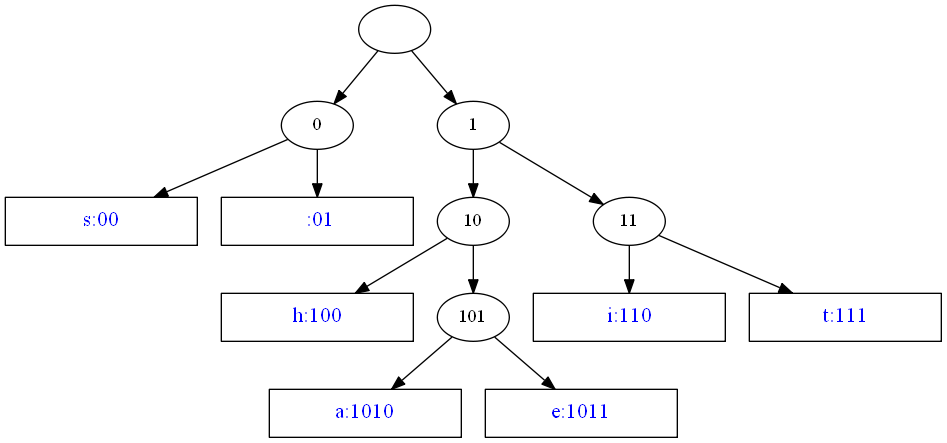
\includegraphics[width=1\textwidth, keepaspectratio]{img/ejemplo.png}}
    \caption{Ejemplo 1}
  \end{figure}
  \begin{figure}[H]
    \centering
    \fbox{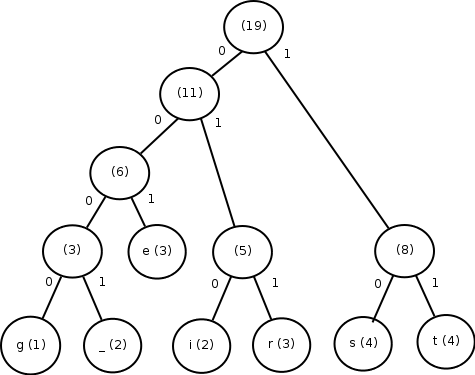
\includegraphics[width=0.9\textwidth, keepaspectratio]{img/ejemplo1.png}}
    \caption{Ejemplo 2}
  \end{figure}

%%%%%%%%%%%%%%%%%%%%
	\newpage
	\subsection{\textcolor{red}{Rúbrica para el contenido del Informe y demostración}}
	\begin{itemize}			
		\item El alumno debe marcar o dejar en blanco en celdas de la columna \textbf{Checklist} si cumplio con el ítem correspondiente.
		\item Si un alumno supera la fecha de entrega,  su calificación será sobre la nota mínima aprobada, siempre y cuando cumpla con todos lo items.
		\item El alumno debe autocalificarse en la columna \textbf{Estudiante} de acuerdo a la siguiente tabla:
	
		\begin{table}[ht]
			\caption{Niveles de desempeño}
			\begin{center}
			\begin{tabular}{ccccc}
    			\hline
    			 & \multicolumn{4}{c}{Nivel}\\
    			\cline{1-5}
    			\textbf{Puntos} & Insatisfactorio 25\%& En Proceso 50\% & Satisfactorio 75\% & Sobresaliente 100\%\\
    			\textbf{2.0}&0.5&1.0&1.5&2.0\\
    			\textbf{4.0}&1.0&2.0&3.0&4.0\\
    		\hline
			\end{tabular}
		\end{center}
	\end{table}	
	

	\end{itemize}

 
	
	\begin{table}[H]
		\caption{Rúbrica para contenido del Informe y demostración}
		\setlength{\tabcolsep}{0.5em} % for the horizontal padding
		{\renewcommand{\arraystretch}{1.5}% for the vertical padding
		%\begin{center}
		\begin{tabular}{|p{2.7cm}|p{7cm}|x{1.3cm}|p{1.2cm}|p{1.5cm}|p{1.1cm}|}
			\hline
    		\multicolumn{2}{|c|}{Contenido y demostración} & Puntos & Checklist & Estudiante & Profesor\\
			\hline
			\textbf{1. GitHub} & Hay enlace URL activo del directorio para el  laboratorio hacia su repositorio GitHub con código fuente terminado y fácil de revisar. &2 &X &2 & \\ 
			\hline
			\textbf{2. Commits} &  Hay capturas de pantalla de los commits más importantes con sus explicaciones detalladas. (El profesor puede preguntar para refrendar calificación). &4 &X &4 & \\ 
			\hline 
			\textbf{3. Código fuente} &  Hay porciones de código fuente importantes con numeración y explicaciones detalladas de sus funciones. &2 &X &2 & \\ 
			\hline 
			\textbf{4. Ejecución} & Se incluyen ejecuciones/pruebas del código fuente  explicadas gradualmente. &2 &X &2 & \\ 
			\hline			
			\textbf{5. Pregunta} & Se responde con completitud a la pregunta formulada en la tarea.  (El profesor puede preguntar para refrendar calificación).  &2 &X &2 & \\ 
			\hline	
			\textbf{6. Fechas} & Las fechas de modificación del código fuente estan dentro de los plazos de fecha de entrega establecidos. &2 &X &2 & \\ 
			\hline 
			\textbf{7. Ortografía} & El documento no muestra errores ortográficos. &2 &X &2 & \\ 
			\hline 
			\textbf{8. Madurez} & El Informe muestra de manera general una evolución de la madurez del código fuente,  explicaciones puntuales pero precisas y un acabado impecable.   (El profesor puede preguntar para refrendar calificación).  &4 &X &4 & \\ 
			\hline
			\multicolumn{2}{|c|}{\textbf{Total}} &20 & &20 & \\ 
			\hline
		\end{tabular}
		%\end{center}
		%\label{tab:multicol}
		}
	\end{table}


%%%%%%%%%%%%%%%%%%%%%%%%%%%%%%%%%%%%%%%%%%%%%%%%%%%%%%%%%%%%%%%%%%%
	
  \newpage
  \section{Referencias}
  \begin{itemize}
    \item \url{https://www.w3schools.com/java/default.asp}
    \item \url{https://www.java.com/es/download/ie_manual.jsp}
    \item \url{https://conclase.net/blog/item/huffman}
  \end{itemize}

%%%%%%%%%%%%%%%%%%%% 
%\clearpage
%\bibliographystyle{apalike}
%\bibliographystyle{IEEEtranN}
%\bibliography{bibliography}
			
\end{document}
